\subsection{SLM}
\subsubsection{Dataset}
The model is trained on Alpaca dataset \cite{alpaca} which is an instruction following dataset which consists of about 52,000 examples of instructions with 4 fields.
\begin{itemize}
	\item \textbf{Instruction: }
	A description of task to be performed
	\item \textbf{Output: }
	Optional contextual or additional information for the task
	\item \textbf{Text: }
	A formatted combination of all components using a standardized template 
\end{itemize} 
This dataset is then prepared for training by selecting instruction, input and output columns and changing the format into the dictionary which created the proper structure for training. 

\subsubsection{Data Preparation and Pipeline}
The dataset is processed to support instruction fine-tuning. The pipeline is designed to handle variable-length sequences. We use a custom instruction Dataset class which pre-tokenizes the data by concatenating the instruction, input, and expected output into a single continuous format:

\begin{verbatim}
	Instruction + Input + ###Response: output
\end{verbatim}

A custom collate function is used to construct training batches where sequences are padded to the maximum length in the batch using the $endoftext$ token with ID 50256. The target values for padded positions are set to an ignore index of -100 so the model does not learn from padding tokens and excludes them from loss calculation. 

\subsubsection{Loading weight and Training configuration}
The model is initialized with pre-trained GPT-2 weights. We implement a custom loading mechanism to map external parameters to the specific PyTorch architecture, where weights are assigned to their corresponding layers. The token embeddings ($wte$) and positional embeddings ($wpe$) are directly mapped to the model embedding layers. The pretrained attention weights ($c_{\text{attn}}$) are split along the last dimension into three distinct components: Query, Key, and Value ($Q, K, V$). The weight matrices for the attention and feed-forward layers are transposed to match PyTorch linear layer expectations.

To train the model, the AdamW optimizer is used to properly handle weight decay, and a low learning rate is applied to fine-tune the model without destabilizing learned representations. The dataset is partitioned using an 85/10/5 split, where training is performed on 85\% of the dataset, testing on 10\%, and validation on 5\%.

\begin{table}[ht]
	\caption{Hyperparameters used for model training}
	\centering
	\begin{tabular}{|l|l|}
		\hline
		\textbf{Hyperparameter} & \textbf{Value} \\
		\hline
		Batch Size &  8\\
		Learning Rate & 5x10-5 \\
		Optimizer & AdamW \\
		Number of Epochs &  5\\
		Weight Decay &  0.1\\
		Max Sequence Length & 1024 tokens \\
		\hline
	\end{tabular}
\end{table}

The training loop evaluates the model on validation set every 5 steps to track convergence and prevent overfitting.

\subsubsection{BPE Tokenizer}
Character level vocabulary is built including all ASCII characters where a special whitespace character Ġ is used. The merging rule is used to combine symbol pairs into sub word tokens. During training, the tokenizer maps each character to its ID and finds the most adjacent pair and replaces occurrences of the pair with new token ID and records the merge until desired vocabulary size is reached. The existing encoder.json vocabulary and vocab.bpe are rules of merging list which assigns each merge a rank so that lower pairs are merged first. During encoding, each chunk is looked up in the vocab and if the chunk is not found then it is passed to the  BPE merger which is split into individual character level token IDs then the merging is done using merge rules from vocab.bpe with accordance to its rank. This process is repeated until no further merges can be performed. The decoding reverses the process converting Ġ back into real spaces and concatenating tokens into readable text.  

\begin{lstlisting}[basicstyle=\footnotesize\ttfamily,caption = Output of BPE Tokenizer on a sample text]
    Input Text : We study in IOE Thapathali #2@ located 
    near Maitighar Mandala.

    Token id: [1135, 2050, 287, 24418, 36, 536, 499, 776, 7344, 
    1303, 17, 31, 5140, 1474, 285, 4548, 394, 283, 6855, 6081]

    Tokenized text: We  study  in  IO E  Th ap ath ali  # 2 @ 
    located near  m ait igh ar  mand ala
\end{lstlisting}

\subsubsection{Data Embedding}
\textbf{Text Embedding}\\
The token IDs are converted into embedding vectors. First the embedding weights are initialized with random values which get changed during the training process. Token embedding provides meaning to the ids. During training tokens dimensions will change so tokens having similar meaning are near to each other in vector space. Embeddings are used to find meanings among the words and not see words as unrelated, random weights. To create embedding vectors a matrix of size $vocab\_size * output\_dim$ is created. If $vocab\_size = 6$ and $output\_dim = 3$ then,

\begin{verbatim}
tensor([[-0.25091976,  0.90142861,  0.46398788],
        [ 0.19731697, -0.68796272, -0.68801096],
        [-0.88383278,  0.73235229,  0.20223002],
        [ 0.41614516, -0.95883101,  0.9398197 ],
        [ 0.66488528, -0.57532178, -0.63635007],
        [-0.63319098, -0.39151551,  0.04951286]], requires_grad=True)
\end{verbatim}


\textbf{Positional Embedding}\\
Self attention mechanism does not have a notion of position or order of tokens within a sequence. Absolute positional embedding is used which is optimized during the training process. For each token ids a vector is created which is than added to previous token embedding and passed to the model.

\begin{figure}[H]
    \centering
    \IfFileExists{Images/SLM/Implementation Details/Embedding.pdf}{%
        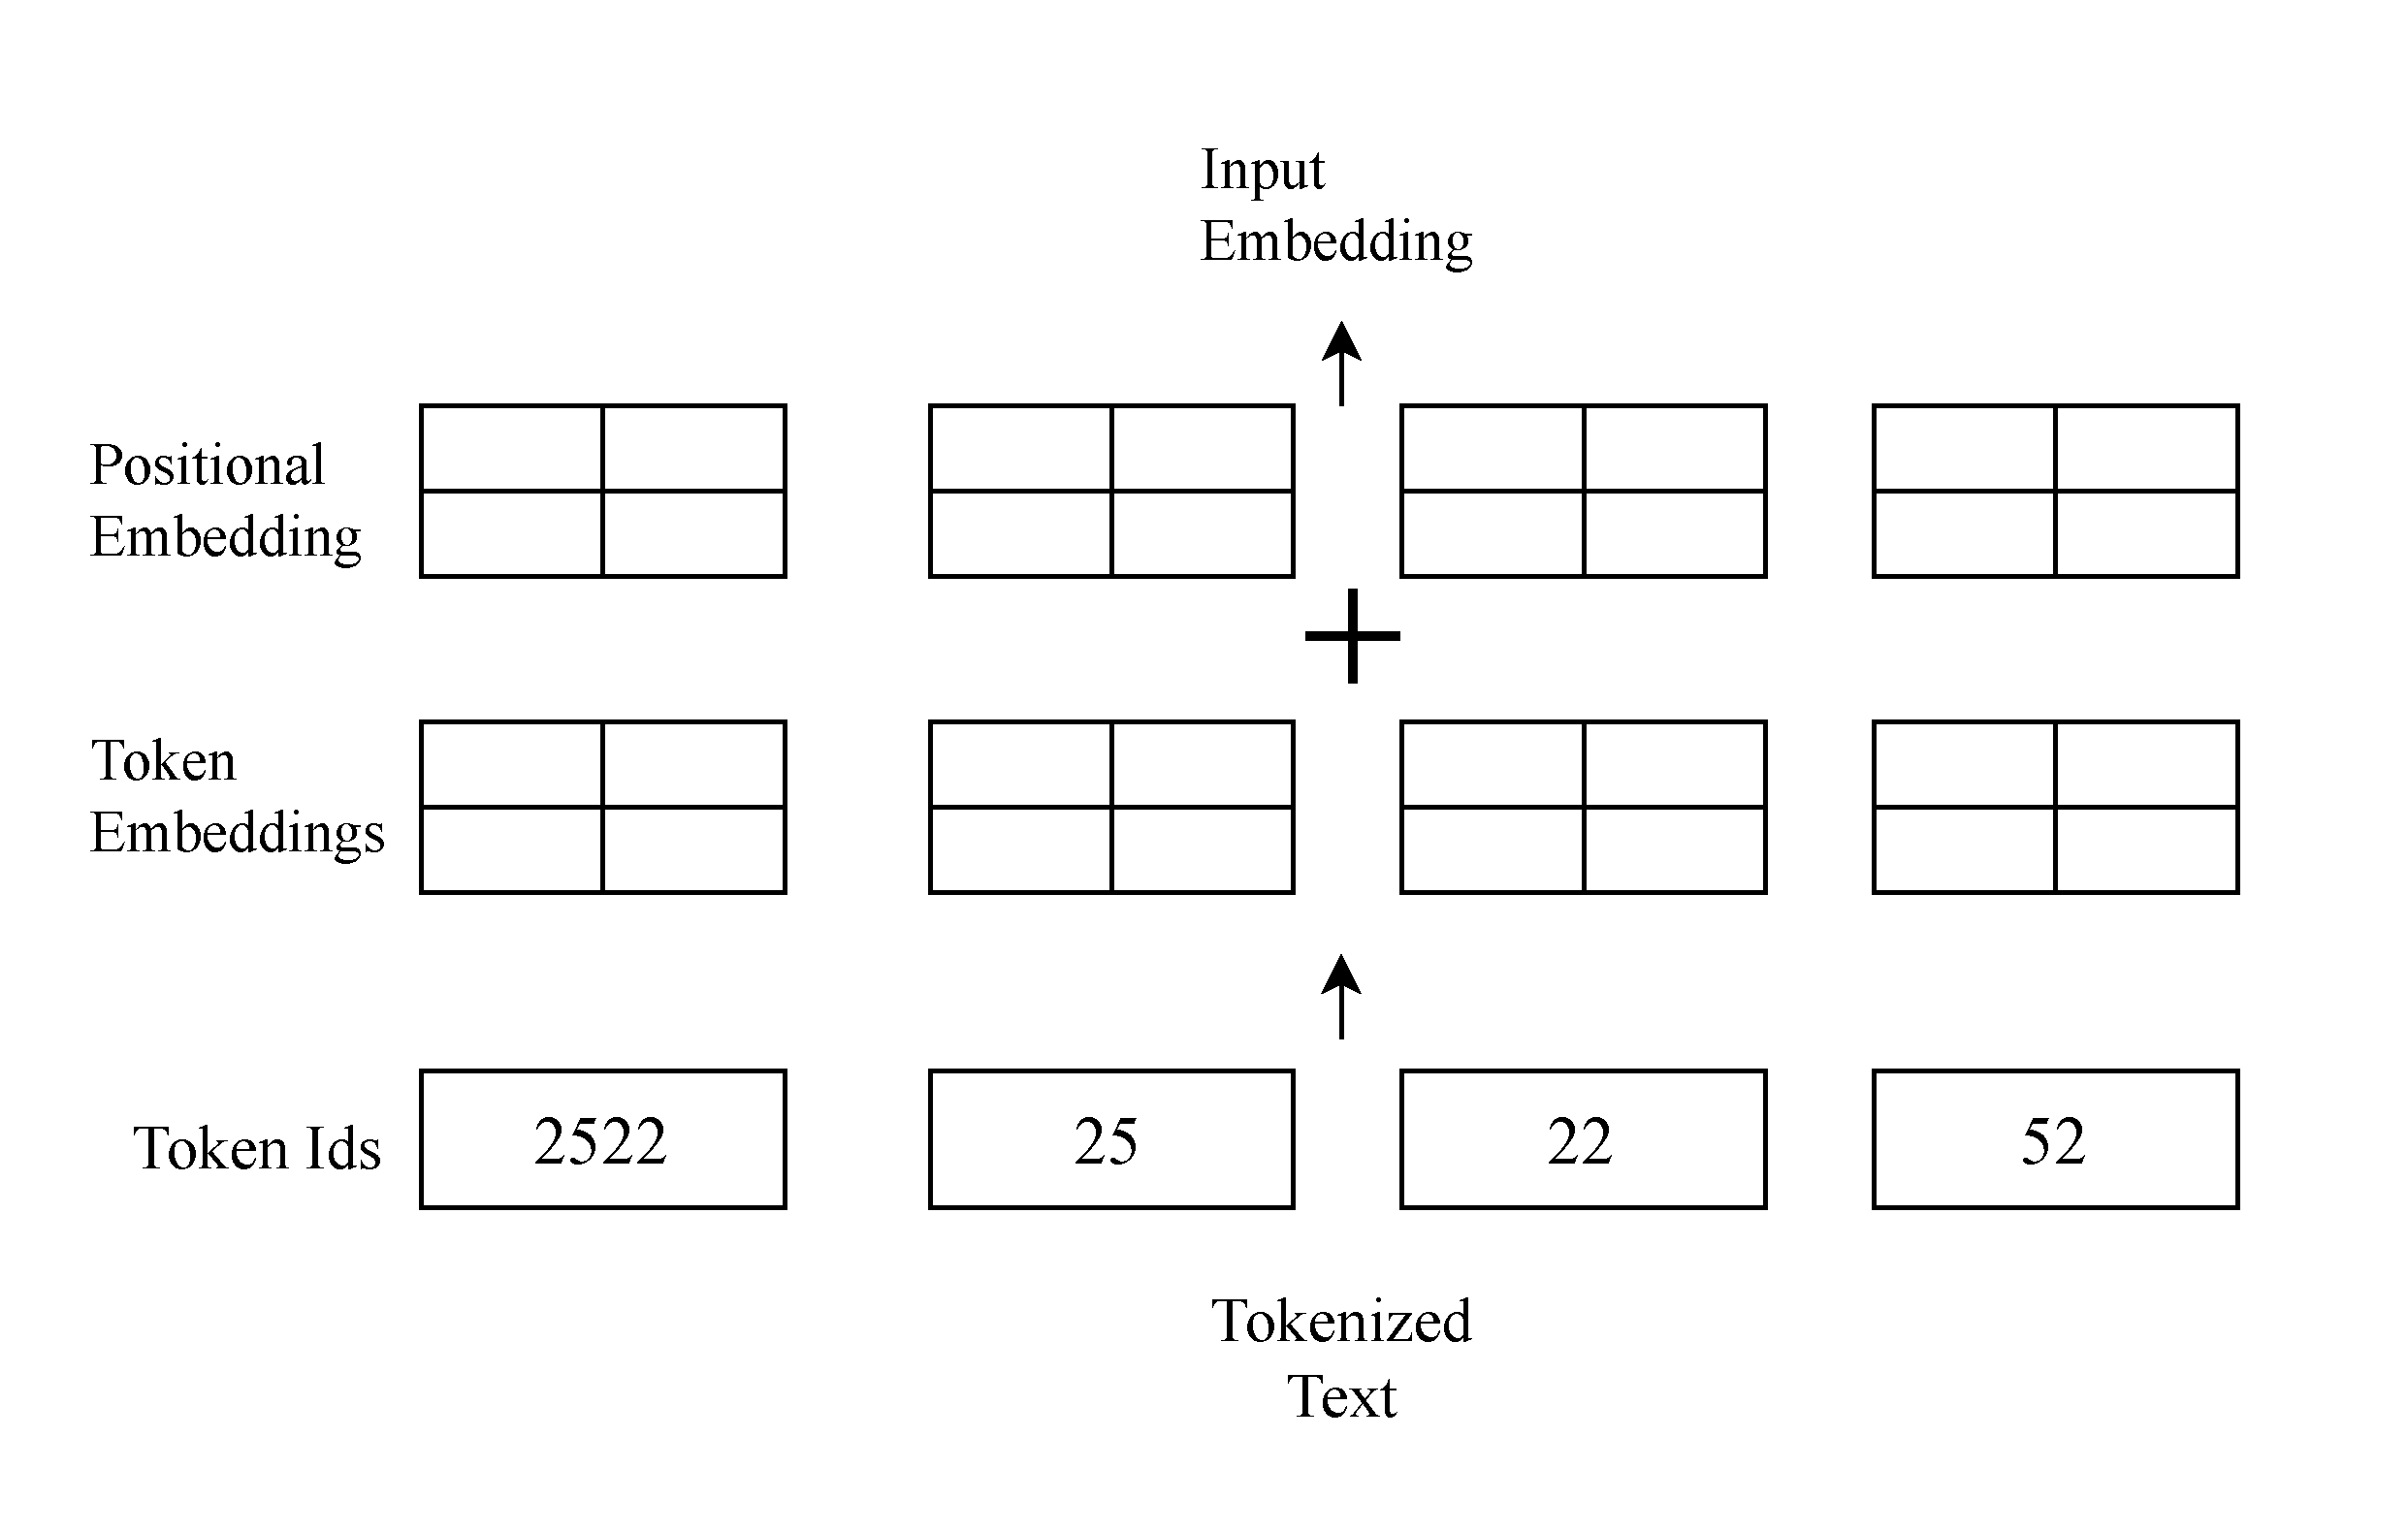
\includegraphics[width=\linewidth]{Images/SLM/Implementation Details/Embedding.pdf}%
    }{%
        \fbox{\parbox{0.92\linewidth}{\centering
        Embedding illustration file not available in the repository.\\
        This figure is intended to show token embeddings combined with positional embeddings before being passed into the decoder.}}%
    }
    \caption{Token and Positional Embedding}
\end{figure}

\subsubsection{Masked Multi-Head Attention Mechanism}
The Multi-Head Attention module uses a casual scaled dot product attention mechanism with multiple heads to create a context vector. 

\begin{figure}[H]
    \centering
    \IfFileExists{Images/SLM/Implementation Details/AttentionMechanism.pdf}{%
        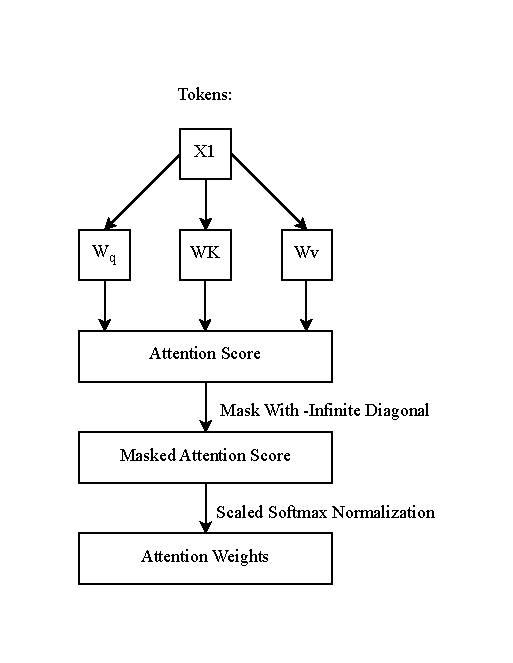
\includegraphics[width=1\linewidth]{Images/SLM/Implementation Details/AttentionMechanism.pdf}%
    }{%
        \fbox{\parbox{0.92\linewidth}{\centering
        Attention mechanism illustration file not available in the repository.\\
        This figure is intended to summarize causal masked multi-head attention with query, key, and value projections.}}%
    }
    \caption{Attention Mechanism}
    \label{fig:Attention Mechanism}
\end{figure}

\begin{itemize}
    \item \textbf{Initialization and projection: }
    The input tensor has shape $(B, T, d_{in})$ where $B$ is the batch size and $T$ is the sequence length. The output dimension $d_{out}$ should be divisible by the number of heads $h$, i.e.,
    $
      d_k = \frac{d_{out}}{h}
    $
    The first three linear layers $W_{\text{query}}, W_{\text{key}}, W_{\text{value}}$ are initialized to project input embeddings into query, key, and value vectors. A causal mask using an upper triangular matrix is applied, ensuring that during training the model attends only to previous positions, preventing information leakage.

    $$Q = XW_Q \quad K = XW_K \quad V = XW_V$$

    The data is projected once and reshaping of resulting tensors is done instead of using separate layers for each head.
    
    \item \textbf{Scaled dot-product attention: }
    First the raw attention scores are calculated by performing matrix multiplication between queries and the transposed keys. To prevent information leakage a casual mask M an upper triangular matrix of negative infinity is used with scores. Then the attention weights are computed by scaling the scores by $\sqrt{d_k}$ and applying a Softmax function:

    \begin{equation}
        \text{Attention}(Q, K, V) = \mathrm{softmax}\!\left(\frac{QK^{T}}{d_k} + M\right)V
    \end{equation}
    The scaling factor $\sqrt{d_k}$ is critical here to counteract the effect of large dot products pushing the Softmax function into regions with extremely small gradients.

    After applying the attention weights to the value vectors V, the resulting context vectors from all h heads are transposed and concatenated to restore the original sequence shape (B,T,$d_{out}$). Finally, a linear output projection W is applied to mix the concatenated representations across heads, yielding the final output of the module.
    
\end{itemize}

\subsubsection{Model Creation}
\textbf{Layer Normalization and GELU activation}\\
For layer normalization which normalizes activations across the embedding dimension for each token independently to compute the mean and variance along the last dimension.

\begin{equation}
\hat{x} = \frac{x - \mu}{\sqrt{\sigma^2 + \epsilon}}, \quad
y = \gamma \hat{x} + \beta
\end{equation}


\begin{table}[ht]
\caption{Model Hyperparameters}
\centering
\begin{tabular}{|l|l|}
\hline
\textbf{Parameter} & \textbf{Value} \\
\hline
Vocabulary Size ($vocab\_size$) & 50257 \\
Context Length ($context\_length$) & 1024 \\
Dropout Rate ($drop\_rate$) & 0.0 \\
QKV Bias ($qkv\_bias$) & True \\
Embedding Dimension ($emb\_dim$) & 768 \\
Number of Layers ($n\_layers$) & 12 \\
Number of Heads ($n\_heads$) & 12 \\
\hline
\end{tabular}
\end{table}

This feed network uses the Gaussian Error Linear Unit (GELU) activation. It introduces non-linearity while allowing small negative values to pass smoothly.

\begin{equation}
\mathrm{GELU}(x) = 0.5 \, x \left[ 1 + \tanh \left( \sqrt{\frac{2}{\pi}} \left( x + 0.044715 \, x^3 \right) \right) \right]
\end{equation}

\textbf{Transformer block and model}\\
The first input goes through layer normalization. The feed forward part consists of two linear layers. The first expands the embedding dimension to 4 times its size, applies GELU and projects the original embedding dimension towards the second linear layer. Which is followed by multi-head attention sub-layer. A dropout is applied to the attention output and a residual connection adds a shortcut. This process is repeated multiple times to form a core transformer stack. The model begins with a token embedding layer and positional embedding of the same dimensions. Which then flows to the stack of n\_layers of the transformer block. A last layer normalization is applied and linear output head is used that projects the embeddings to a vocabulary size. The result logits represents unnormalized probabilities over next token for each position in the sequence.
